\documentclass[12pt]{article}
\usepackage[utf8]{inputenc}
\usepackage{listings}
\usepackage[margin=1in]{geometry}
\usepackage{graphicx} % graficos
\usepackage{setspace}
\usepackage{xcolor}
\usepackage{color}
\usepackage{listings}

\graphicspath{ {/home/giovanni/famaf/2014/Modelos-y-Simulacion/trabajo_especial_I/informe/figuras/} }

\title{Modelos y Simulaci\'on}
\author{Giovanni Rescia \\ \\ \large FaMAF}
\date{21 de Mayo de 2014}

\begin{document}

\maketitle
\pagebreak

\noindent El siguiente gr\'afico podemos observar el estado del sistema actual:

\begin{figure}[hbt]
\noindent\makebox[\textwidth]{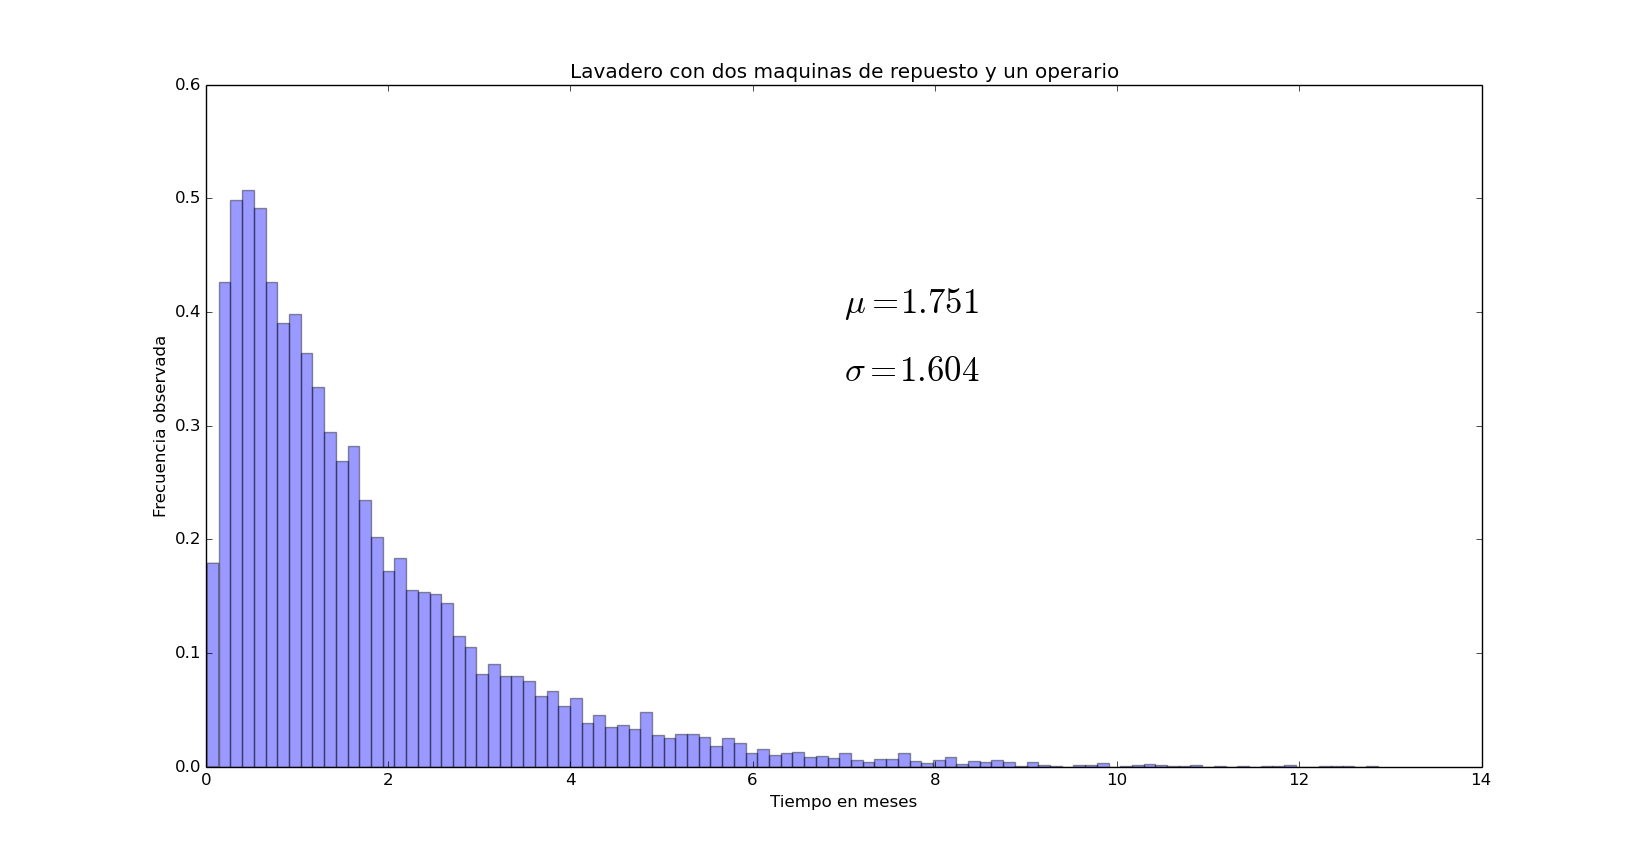
\includegraphics[scale=0.4]{figure_1}}
\end{figure}
Este ser'ia el segundo p'arrafo.
Y aqu'i puedes escribir m'as cosas.
Mi primer documento en \LaTeX{}.

\end{document}